\chapter{Representation of a Gaussian phase space distribution by concentric ellipses of macroparticles}

For a Gaussian phase space distribution, the contours of constant density lie on concentric ellipses.  We wish to represent this phase space by a series of concentric ellipses on which macroparticles are evenly spaced.  This puts more macroparticles at the edges of the distribution than a method with equally-weighted particles does, which helps us observe nonlinear effects on the beam.

\section{Representing an ellipse in phase space}

\subsection{Action-angle variables}
The transformation from an action-angle variable representation $(J,\phi)$ to phase space coordinates $(x, x')$ is given by
\Begineq
	\begin{pmatrix} x \\ x' \end{pmatrix}
	= \sqrt{2J} 
	\begin{pmatrix} \sqrt{\beta} & 0 \\ -\frac{\alpha}{\sqrt{\beta}} & -\frac{1}{\sqrt{\beta}} \end{pmatrix}
	\begin{pmatrix} \cos\phi \\ \sin\phi \end{pmatrix}.
\Endeq
where $\beta$, $\alpha = -\frac{\beta'}{2}$, and $\gamma = \frac{1+\alpha^2}{\beta}$ are the Twiss parameters.  Holding these parameters and $J$ constant and iterating $\phi$ between $0$ and $2\pi$ defines an ellipse centered at the origin.  $J = \frac{1}{2}[\gamma x^2 + 2 \alpha x x' + \beta x'^2]$ is called the Courant-Snyder invariant, and it is proportional to the internal area of the ellipse: $A = 2\pi J$. 

\textit{Sidenote}: it can be shown that this transformation is canonical because the Jacobian matrix $\mathbf{M} = \frac{\partial(x,x')}{\partial(J,\phi)}$ is symplectic ($\mathbf{M}\mathbf{J}\mathbf{M}^T = \mathbf{J}$ for $\mathbf{J} = (\begin{smallmatrix} 0 && 1 \\ -1 && 0 \end{smallmatrix})$).


\begin{figure}[htp]
	\centering \includegraphics[scale=0.75]{phaseellipse.eps}
	\caption{Anatomy of a phase space ellipse.  Modified from: H. Wiedemann, Particle Accelerator Physics I, 2nd ed., p.152.}
	\label{fig:ellipse}
\end{figure}

\section{The Gaussian distribution}
For a distribution of particles in phase space with density $\rho(J,\phi)$, we define the emittance to be
\Begineq
	\varepsilon = \langle J \rangle = \int dJ \, d\phi \, J\rho(J,\phi).
\Endeq
In these $(J,\phi)$ coordinates, a Gaussian phase space distribution can be represented as
\Begineq
	\rho(J,\phi) = \frac{1}{2\pi\varepsilon} e^{-\frac{J}{\varepsilon}}.
	\label{eq:rho}
\Endeq

This distribution is normalized to 1, i.e. $\int dJ \, d\phi \rho(J,\phi) = 1$.  Its emittance is $\varepsilon$, since
\Begineq
	\langle J \rangle = \int_{0}^{\infty} dJ \int_{0}^{2\pi} d\phi \, J \rho(J,\phi) = \frac{1}{\varepsilon} \int_{0}^{\infty} dJ \, J e^{-\frac{J}{\varepsilon}} = \varepsilon.
\Endeq
The rms beam size and divergence are
\begin{align}
	\sigma_x & = \sqrt{\langle x^2 \rangle} = \sqrt{\langle 2J\beta \cos^2 \phi \rangle} = \sqrt{\varepsilon\beta}  \\
	\sigma_{x'} & = \sqrt{\langle x'^2 \rangle} = \sqrt{\biggl\langle \frac{2J}{\beta} (\alpha \cos\phi + \sin\phi)^2 \biggr\rangle} = \sqrt{\varepsilon\gamma},
	\label{eq:rms}
\end{align}
while the covariance is
\Begineq
	\langle xx' \rangle = \langle -2J (\alpha \cos^2 \phi + \sin\phi \cos\phi) \rangle = -\varepsilon\alpha.
	\label{eq:corr}
\Endeq

\subsection{Alternate representation of the distribution}
Equations (\ref{eq:rms}) and (\ref{eq:corr}) lead to an alternative representation of the distribution, which replaces the Twiss parameters with rms quantities.
From the definition of $\gamma$, 
\Begineq
	\langle x'^2 \rangle = \varepsilon\frac{1+\alpha^2}{\beta} = \frac{\varepsilon^2 + \langle xx' \rangle^2}{\langle x^2 \rangle} \quad \Rightarrow \quad \varepsilon = \sqrt{\langle x^2 \rangle\langle x'^2 \rangle - \langle xx' \rangle^2}.
\Endeq
So, the distribution can be written
\Begineq
	\rho(x,x') = \frac{1}{2\pi\sqrt{\langle x^2 \rangle\langle x'^2 \rangle - \langle xx' \rangle^2}} \exp \left( -\frac{\langle x'^2 \rangle x^2 - 2 \langle xx' \rangle xx' + \langle x^2 \rangle x'^2}{2(\langle x^2 \rangle\langle x'^2 \rangle - \langle xx' \rangle^2)} \right)
\Endeq

\subsection{Implementation}
\begin{figure}[htp]
	\centering \includegraphics[scale=0.75]{filledellipse.eps}
	\caption{We partition the phase space into regions bounded by ellipses (solid ellipses in red), and then calculate where to place the particles (dots in blue).  The red ellipses are placed so that their $\sqrt{J}$ increases by regular steps.  A number of blue ellipses of particles cover the region inside a certain cutoff radius, and one blue ellipse covers the region outside the largest red ellipse.  For this example, we set the cutoff at 3$\sigma$, have 3 ellipses in the inner region, and have 50 particles per ellipse.}
	\label{fig:finishedellipse}
\end{figure}

\begin{itemize}
\item Since we cannot represent the distribution with an infinite number of ellipses, we must implement some sort of sigma cutoff $g$ at which we will stop representing the distribution regularly --- commonly, $g$ is set to $3$ or $4$.  The space inside this sigma cutoff will be represented by a set of $N$ concentric ellipses; the space outside will be represented by a single ellipse.
\item Partition the inner region into $N$ sections $\lbrace S_{n} \rbrace, 1 \leq n \leq N$, each bounded by concentric boundary ellipses at $J = B_{n-1}$ and $B_{n}$, which will be calculated below.  $\sqrt{J}$ is increased by a constant amount from one boundary to the next, i.e. $\sqrt{B_{n}} = n\Delta$, $n = 0,...,N$.  Including the exterior section $S_{out}$, there are $N+1$ sections.
\item In each section $S_{n}$, place an ellipse of $M$ macroparticles at $J = J_{n}$.  Also place an ellipse at $J = J_{out}$ in $S_{out}$.  The macroparticles will be placed uniformly in $0 \leq \phi < 2\pi$.
\end{itemize}

The goal is to replace the Gaussian distribution given in equation \ref{eq:rho} with 
\Begineq
	\rho_{model}(J,\phi) = \left[ \sum_{n=1}^{N} q_{n} \, \delta(J - J_{n}) + q_{out} \, \delta(J - J_{out}) \right] \, \sum_{m=1}^{M} \frac{1}{M} \, \delta(\phi - 2\pi \frac{m}{M})
\Endeq
where each ring has a total weight $q_{n}$.  

We determine $\lbrace q_{n} \rbrace$, $\lbrace J_{n} \rbrace$, $q_{out}$, and $J_{out}$ by requiring that these conditions be satisfied:
\begin{itemize}
\item $\rho_{model}$ is normalized to 1,
\item $\langle J \rangle_{model} = \varepsilon$ for the entire distribution,
\item $q_{n} = \iint_{S_{n}} dJ d\phi \, \rho$ and $\langle J \rangle_{n} = \iint_{S_{n}} dJ d\phi \, J \rho$ agree between the model and Gaussian distributions, for each section $S_{n}$
\end{itemize}
That is, each ring carries the same weight and $\langle J \rangle$ as the section it represents, and the distribution as a whole has the same normalization and emittance.  In our partitioning, we are effectively doing the following:
\begin{align}
	1 & = \int_{0}^{\infty} dJ \int_{0}^{2\pi} d\phi \, \rho(J,\phi)                                                                                         \\
	  & = \sum_{n=1}^{N} \underbrace{\int_{B_{n-1}}^{B_{n}} dJ \int_{0}^{2\pi} d\phi \, \rho(J,\phi)}_{q_{n}} + \underbrace{\int_{B_{N}}^{\infty} dJ \int_{0}^{2\pi} d\phi \, \rho(J,\phi)}_{q_{out}}                                                                                                          \\
	\langle J \rangle & = \int_{0}^{\infty} dJ \int_{0}^{2\pi} d\phi \, J \, \rho(J,\phi)                                                                    \\
	                  & = \sum_{n=1}^{N} \underbrace{\int_{B_{n-1}}^{B_{n}} dJ \int_{0}^{2\pi} d\phi \, J \, \rho(J,\phi)}_{\langle J \rangle_{n}} + \underbrace{\int_{B_{N}}^{\infty} dJ \int_{0}^{2\pi} d\phi \, J \, \rho(J,\phi)}_{\langle J \rangle_{out}}.
\end{align}


The boundary ellipses lie at $J \in \lbrace B_{n} \rbrace, 0 \leq n \leq N$, where $B_{0} = 0$ characterizes the origin of the phase space coordinates.  If our sigma cutoff is $g$, the outermost boundary is defined by $\sqrt{B_{N}} = g \sqrt{\frac{\varepsilon}{2}}$, so
\Begineq
	B_{n} = g^2 \frac{n^2}{N^2} \frac{\varepsilon}{2}.
\Endeq

The requirement that, for each section, $q_n$ is the same for the model and the Gaussian distribution leads to 
\Begineq\begin{split}
	q_{n} & = \int_{B_{n-1}}^{B_{n}} dJ \int_{0}^{2\pi} d\phi \, \rho(J,\phi) = \frac{1}{\varepsilon} \int_{B_{n-1}}^{B_{n}} dJ \, e^{-\frac{J}{\varepsilon}} = \exp \left( -\frac{B_{n-1}}{\varepsilon} \right) - \exp \left( -\frac{B_{n}}{\varepsilon} \right),  \\
	q_{out} & = \int_{B_{N}}^{\infty} dJ \int_{0}^{2\pi} d\phi \, \rho(J,\phi) = \exp \left( -\frac{B_{N}}{\varepsilon} \right).
\end{split}\Endeq

The same constraint on $\langle J \rangle_n$ leads to
\Begineq\begin{split}
	q_{n}J_{n} & = \int_{B_{n-1}}^{B_{n}} dJ \, J \, \frac{1}{\varepsilon} e^{-\frac{J}{\varepsilon}} = \varepsilon \int_{\frac{B_{n-1}}{\varepsilon}}^{\frac{B_{n}}{\varepsilon}} d\xi \, \xi \, e^{-\xi} = \varepsilon (\xi + 1) e^{-\xi} \biggr\vert_{\frac{B_{n}}{\varepsilon}}^{\frac{B_{n-1}}{\varepsilon}},                              \\
	q_{out}J_{out} & = \int_{B_{N}}^{\infty} dJ \, J \, \frac{1}{\varepsilon} e^{-\frac{J}{\varepsilon}} = \varepsilon (\xi + 1) e^{-\xi} \biggr\vert_{\xi = \frac{B_{n}}{\varepsilon}}.
\end{split}\Endeq

\section{Final Results}
Our model distribution is
\Begineq
	\rho_{model}(J,\phi) = \left[ \sum_{n=1}^{N} q_{n} \, \delta(J - J_{n}) + q_{out} \, \delta(J - J_{out}) \right] \, \sum_{m=1}^{M} \frac{1}{M} \, \delta(\phi - 2\pi \frac{m}{M}).
\Endeq

Also, let us use dimensionless quantities $b_{n} = \frac{B_{n}}{\varepsilon} = \frac{g^2 n^2}{2 N^2}$.  The weight of each macroparticle is
\Begineq
	q_{n}/M = \frac{1}{M}(e^{-b_{n-1}} - e^{-b_{n}}),
\Endeq
\Begineq
	q_{out}/M = \frac{1}{M} e^{-b_{N}}.
\Endeq
The rings lie at positions
\Begineq
	J_{n} = \varepsilon \, \frac{(b_{n-1}+1) e^{-b_{n-1}} - (b_{n}+1) e^{-b_{n}}}{e^{-b_{n-1}} - e^{-b_{n}}},
\Endeq
\Begineq
	J_{out} = \varepsilon (b_{N}+1).
\Endeq

